% Document setup
\RequirePackage{fix-cm}
\documentclass{article}
\usepackage{preamble}

%===============================%
%=============Inputs============%
%===============================%
\newcommand{\studentname}{YOUR NAME GOES HERE!}

%===============================%
%====Make Solutions Visible=====%
%===============================%
\showsolutionstrue

%===============================%
%=============Figures===========%
%===============================%
% Remember to start figures with 
% \begin{figure}[H]
% the [H] is critical


%==============================%
%=====Beginning of Document====%
%==============================%
\begin{document}
\pagestyle{mypagestyle}


%%%%%%%%%%%%%%%%%%%%%%%%%%%%%%%%%%%%%%%%%%%%%%%%%%%%%%%%%%%%%%%%%%%%%%%%%%%%%%%%%%%%%%%%%%%%%%%%%%%%%%%%%%%%%%%%%%%%%%%%%%
% Project 1: Newton's Method and Genetic Algorithm
%%%%%%%%%%%%%%%%%%%%%%%%%%%%%%%%%%%%%%%%%%%%%%%%%%%%%%%%%%%%%%%%%%%%%%%%%%%%%%%%%%%%%%%%%%%%%%%%%%%%%%%%%%%%%%%%%%%%%%%%%%
\project{1}{Newton's Method and Genetic Algorithm (50 points)}{Tuesday, Feb 10th @ 11:59 PM PST}[Add instructions]


\begin{itemize} 

\item{\textbf{Learning Goal}: understanding classical optimization and genetic machine-learning.}

\item{\textbf{Abstract}: This project is designed to highlight the very basics of optimization and machine-learning.  
There are two parts: (1) classical gradient-based optimization and (2) genetic machine learning algorithms.}
\item{\textbf{Reading}: 
This project directly corresponds to Chapter 1 in the \href{https://bcourses.berkeley.edu/courses/1547162/files/folder/Course%20Reader?preview=92339267}{course reader}.} 

\begin{figure}[h]
\centering
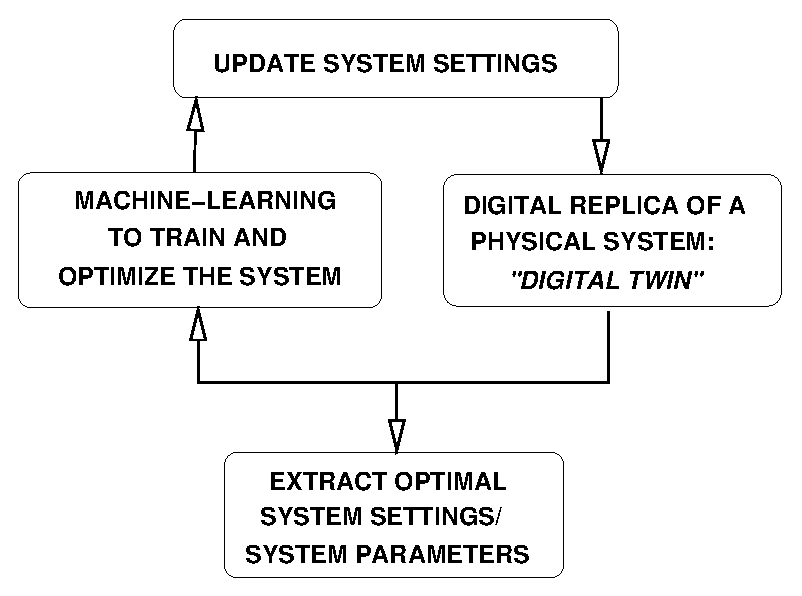
\includegraphics[width=0.6\textwidth]{figures/MACHINE-LEARNING-DIGITAL-TWIN.eps}
\caption{Machine-learning and digital-twin models.}
\label{tarek-project-1}
\end{figure}

\end{itemize} 

\begin{enumerate}
%%%%%%%%%%%%%%%%%%%%%%%%%%%%%%%%%%%%%%%%%%%%%%%%%%%%%%%%%%%%%%%%%%%%%%%%%%%%%%%%%%%%%%%%%%%%%%%%%%%%%%%%%%%%%%%%%%%%%%%%%%
% Problem 1
%%%%%%%%%%%%%%%%%%%%%%%%%%%%%%%%%%%%%%%%%%%%%%%%%%%%%%%%%%%%%%%%%%%%%%%%%%%%%%%%%%%%%%%%%%%%%%%%%%%%%%%%%%%%%%%%%%%%%%%%%%
\newpage
\item {\bf Newton's Method. (20 points)} In mathematics, we optimize a function $f(x)$ by choosing from a set of candidate inputs $x$ and finding the $x$ which either maximizes or minimizes $f(x)$, sometimes under a set of constraints. In this course, we will simply refer to these functions as {\it cost functions} or {\it objective functions}, $\Pi(x)$.

In advanced manufacturing, cost functions are often non-convex in the design parameter space and often non-smooth, so their optimization is usually difficult with direct application of gradient methods. As a reference point, however, in this problem you will code Newton's method, a gradient-based method for later comparison to the genetic algorithm.

The two objective functions to be minimized in this assignment are:
\begin{align}
\Pi_{a}(x) &= x^{2} \\
\Pi_{b}(x) &= \left( x + \frac{\pi}{2}\sin(x) \right)^{2}
\end{align}

\begin{enumerate}

%%%%%%%%%%%%%%%%%%%%%%%%%%%%%%%
% Problem 1a
%%%%%%%%%%%%%%%%%%%%%%%%%%%%%%%
\item Plot both objective functions on the same axes on the domain $-20 \leq x \leq 20$.

% \begin{answer}
% %-----------------------------%
% % Place answer here
% %-----------------------------%
% \end{answer}

%%%%%%%%%%%%%%%%%%%%%%%%%%%%%%%
% Problem 1b
%%%%%%%%%%%%%%%%%%%%%%%%%%%%%%%
\item Write a function to use Newton's Method, with the syntax
\begin{code}
def myNewton(f, df, x0, TOL, maxit): 
    # Your code goes here
    return (sol, its, hist)
\end{code}

where
\begin{itemize}
\item \verb|sol|:   $M \times 1$ array, the final value of the independent variable $x$.
\item \verb|its|:   scalar, the number of iterations performed.
\item \verb|hist|:  $M \times(\verb|its|+1)$ array, where $\verb|hist(:, i + 1)| = x_{i}$. 
\item \verb|f|:     function with input size $M \times 1$ and output size $M \times 1$, gradient of $\Pi$.
\item \verb|df|:    function with input size $M \times 1$ and output size $M \times M$, Hessian of $\Pi$.
\item \verb|x0|:    $M \times 1$ array, initial guess to start iterations.
\item \verb|TOL|:   scalar, maximum allowable distance of \verb|f(sol)| from 0.
\item \verb|maxit|: scalar, maximum allowable iterations.
\end{itemize}

$M$ (the dimension of function input $x$) equals 1 in this problem.

% \begin{answer}
% %-----------------------------%
% % Place answer here
% %-----------------------------%
% \end{answer}


%%%%%%%%%%%%%%%%%%%%%%%%%%%%%%%
% Problem 1c
%%%%%%%%%%%%%%%%%%%%%%%%%%%%%%%
\item Provide your code for $f$ and $df$ corresponding to $\Pi_{a}$ and $\Pi_{b}$. Make two plots: 1.) Plot $d\Pi_{a}/dx$ and $d\Pi_{b}/dx$ (plotting functions $f$) on the domain $-20 \leq x \leq 20$. 2.) Plot $d^2\Pi_{a}/dx^2$ and $d^2\Pi_{b}/dx^2$ (plotting functions $df$) on the domain $-20 \leq x \leq 20$.

% \begin{answer}
% %-----------------------------%
% % Place answer here
% %-----------------------------%
% \end{answer}

%%%%%%%%%%%%%%%%%%%%%%%%%%%%%%%
% Problem 1d
%%%%%%%%%%%%%%%%%%%%%%%%%%%%%%%
\item Use \verb|myNewton()| to minimize $\Pi_{a}$ and $\Pi_{b}$, with \verb|x0| = $2 \times 10^{k}$, for $k\in\{ -1, 0, 1 \}$. Use \verb|TOL| = $10^{-8}$ and \verb|maxit| = 20. Plot $\Pi(\verb|hist|)$ for $\Pi_{a}$ and $\Pi_{b}$. Explain any significant results.

% \begin{answer}
% %-----------------------------%
% % Place answer here
% %-----------------------------%
% \end{answer}

\end{enumerate}


\newpage
%%%%%%%%%%%%%%%%%%%%%%%%%%%%%%%%%%%%%%%%%%%%%%%%%%%%%%%%%%%%%%%%%%%%%%%%%%%%%%%%%%%%%%%%%%%%%%%%%%%%%%%%%%%%%%%%%%%%%%%%%%
% Problem 2
%%%%%%%%%%%%%%%%%%%%%%%%%%%%%%%%%%%%%%%%%%%%%%%%%%%%%%%%%%%%%%%%%%%%%%%%%%%%%%%%%%%%%%%%%%%%%%%%%%%%%%%%%%%%%%%%%%%%%%%%%%
\item {\bf Genetic Algorithm. (30 points)} Please note that your GA code will be employed multiple times in future projects; the more time you spend making it more general the less time you will spend modifying it for all future assignments. 

\begin{enumerate}
%%%%%%%%%%%%%%%%%%%%%%%%%%%%%%%
% Problem 2a
%%%%%%%%%%%%%%%%%%%%%%%%%%%%%%%
\item Write a genetic algorithm in terms of the general parameters:

Input
\begin{itemize}
\item \verb|S|:   scalar, the number of total design strings per generation.
\item \verb|P|:   scalar, the number of design strings to preserve and breed.
\item \verb|K|:   scalar, the number of offspring.
\item \verb|TOL|: scalar, the acceptable cost function threshold to stop evolution.
\item \verb|G|:   scalar, maximum total generations (terminates code if \verb|TOL| is not reached). 
\item \verb|dv|:  scalar, the number of design variables per string.
\item \verb|lim|:  $\verb|dv| \times \verb|2|$ , the lower and upper limits for each design variable.
\end{itemize}

Recommended outputs
\begin{itemize}
\item \verb|Pi|: $\verb|G| \times \verb|S|$ array, where \verb|Pi(g, s)| is the cost of the \verb|s|'th-ranked design in the \verb|g|'th generation.
\item \verb|Pi_min|: $1 \times \verb|G|$ array, where \verb|Pi_min(g)| is the minimum cost in the \verb|g|'th generation.
\item \verb|Pi_avg|: $1 \times \verb|G|$ array, where \verb|Pi_avg(g)| is the average cost in the \verb|g|'th generation.
% \item \verb|Orig|: $\verb|G| \times \verb|S|$ array, where \verb|Orig(g, :)| represents the indices of each sorted entry from before they were sorted. (Hint: See MATLAB's \verb|sort()| function.
\item \verb|Lambda|: $\verb|S| \times \verb|dv|$ array of the most recent generation's design strings.
\end{itemize}

\vspace{3mm}
Debug your code on $\Pi_{a}$ and $\Pi_{b}$ using parameters \verb|S| = 50, \verb|P| = 12, \verb|K| = 12, \verb|lim| = \mbox{[-20, 20]}, \verb|dv| = 1, $\verb|TOL| = 10^{-6}$, nearest-neighbor breeding as outlined in the notes, no mutations, no inbreeding prevention, and a total of  \verb|G| = 100 generations. Provide your code below.

% \begin{answer}
% %-----------------------------%
% % Place answer here
% %
% % NOTE! For typesetting code in
% % LaTeX, we provide a code environment
% %
% % For example:
% %-----------------------------%

% We recommend using the \verb|code| environment for MATLAB or Python code. Here is an example of how to use it:

% \begin{code}[matlab][MATLAB Code]
% >> disp('Hello World!')
% \end{code}

% \begin{code}[python][Python Code]
% print('Hello World!')
% \end{code}

% \end{answer}

%%%%%%%%%%%%%%%%%%%%%%%%%%%%%%%
% Problem 2b
%%%%%%%%%%%%%%%%%%%%%%%%%%%%%%%
\item Attempt to minimize $\Pi_{b}$ from problem 1 using your GA to a tolerance of $\Pi_{b}(x) \leq \verb|TOL| = 10^{-6}$. Use the same GA parameters as outlined in part (a) for debugging your code. Plot the cost of the best design and the mean cost of all of the design strings for each generation on a log-log or semilog plot. Based on this plot, what observations can you make about the diversity of genetic fitness from one generation to the next and across the entire simulation?
% \begin{answer}
% %-----------------------------%
% % Place answer here
% %-----------------------------%
% \end{answer}

%%%%%%%%%%%%%%%%%%%%%%%%%%%%%%%
% Problem 2c
%%%%%%%%%%%%%%%%%%%%%%%%%%%%%%%
\item What would the case with zero parents represent (genetic information does not make it to the new generation)? How would it perform? Conduct a trial or theorize about its run time and reliability.
% \begin{answer}
% %-----------------------------%
% % Place answer here
% %-----------------------------%
% \end{answer}

%%%%%%%%%%%%%%%%%%%%%%%%%%%%%%%
% Problem 2d
%%%%%%%%%%%%%%%%%%%%%%%%%%%%%%%
\item Research question: Discuss the advantages and disadvantages of using Newton's method and a genetic algorithm for global optimization of complicated functions. When is each method useful? Think particularly about run time, reliability and the limitations on the conditions a function must satisfy for each method to work.
% \begin{answer}
% %-----------------------------%
% % Place answer here
% %-----------------------------%
% \end{answer}

\end{enumerate}



\end{enumerate}




% End document
\end{document}